%%%%%%%%%%%%%%%%%%%%%%%%%%%%%%%%%%%%%%%%%%%%%%%%%%%%%%%%%%%%%%%%%%%%%%
% LaTeX Template: Beamer arrows
%
% Source: http://www.texample.net/
% Feel free to distribute this template, but please keep the
% referal to TeXample.net.
% Date: Nov 2006
% 
%%%%%%%%%%%%%%%%%%%%%%%%%%%%%%%%%%%%%%%%%%%%%%%%%%%%%%%%%%%%%%%%%%%%%%

\documentclass{beamer} %
\usetheme{Heidelberg}
\usepackage[utf8]{inputenc}
\usepackage[T1]{fontenc}
\usepackage{lmodern}
%\usefonttheme{professionalfonts}
%\usepackage{times}

\usepackage{tikz}
\usepackage{amsmath}
\usepackage{verbatim} % For the comment environment.
\usepackage{graphicx}
\usepackage{algpseudocode} % For the 'algorithmic' environment.
\usepackage{algorithm} % For the floating 'algorithm' environment.

\usepackage{listings} % For displaying code.

\lstdefinelanguage{JavaScript}{
  keywords={typeof, new, true, false, catch, function, return, null, catch, switch, var, if, in, while, do, else, case, break},
  keywordstyle=\color{blue}\bfseries,
  ndkeywords={class, export, boolean, throw, implements, import, this},
  ndkeywordstyle=\color{darkgray}\bfseries,
  identifierstyle=\color{black},
  sensitive=false,
  comment=[l]{//},
  morecomment=[s]{/*}{*/},
  commentstyle=\color{purple}\ttfamily,
  stringstyle=\color{red}\ttfamily,
  morestring=[b]',
  morestring=[b]"
}

\lstset{
    basicstyle=\footnotesize\ttfamily,
    language=JavaScript,
    breaklines=true,
    showtabs=true,
    showspaces=false,
    showstringspaces=false,
    tabsize=4,
    inputencoding=utf8,
    literate={ä}{{\"a}}1 {ö}{{\"o}}1 {ü}{{\"u}}1 {ß}{{\ss}}1 {²}{{$^2$}}1 {ð}{{\dh}}1 {ó}{{\'o}}1 {á}{{\'a}}1
}

\author{Rebekka Hubert \and Michael Staniek \and Simon Will}
\title{Annotation als Suche}

\begin{document}

\begin{comment}
    :Title: Beamer arrows
    :Tags: Remember picture, Beamer, Physics & chemistry, Overlays
    :Use page: 3

    With PGF/TikZ version 1.09 and later, it is possible to draw paths between nodes across
    different pictures. This is a useful feature for presentations with the
    Beamer package. In this example I've combined the new PGF/TikZ's overlay feature
    with Beamer overlays. Download the PDF version to see the result.

    **Note.** This only works with PDFTeX, and you have to run PDFTeX twice.

    | Author: Kjell Magne Fauske

\end{comment}

% For every picture that defines or uses external nodes, you'll have to
% apply the 'remember picture' style. To avoid some typing, we'll apply
% the style to all pictures.
\tikzstyle{every picture}+=[remember picture]

% By default all math in TikZ nodes are set in inline mode. Change this to
% displaystyle so that we don't get small fractions.
\everymath{\displaystyle}

\maketitle

\begin{frame}
    \frametitle{Übersicht}
    \tableofcontents
\end{frame}

\section{Motivation}

\begin{frame}
    \frametitle{Motivation}
    \begin{itemize}
        \item Menschliche Annotation
            \begin{itemize}
                \item dauert und kostet
                \item bei Dependenzparses immer noch ungeschlagen. % OK, aber es wird ja auch am Menschen evaluiert …
            \end{itemize}
        \item Wir suchen eine Möglichkeit, Annotatoren zu unterstützen
            \begin{itemize}
                \item Basierend auf vielen möglichen Parses für einen Satz Fragen an den Annotator stellen
                \item anhand der Fragen zum optimalen Parsebaum gelangen
            \end{itemize}
    \end{itemize}
\end{frame}

\begin{frame}
    \frametitle{Für wen?}
    \begin{itemize}
        \item Das Programm soll für Annotatoren gedacht sein. 
            \begin{itemize}
                \item Diese Userklasse hat nicht unbedingt viel Programmiererfahrung.
            \end{itemize}
        \item Eine gewisse Grunderfahrung im Annotieren wird vorausgesetzt.
    \end{itemize}
\end{frame}

\begin{frame}
    \section{Requirements}
    \frametitle{Requirements}
    Um die Anpassungsfähigkeit des Systems nicht von Anfang an einzuschränken, bietet es sich an, das System in drei Module aufzuteilen:
    \begin{itemize}
        \item Preprocessing: 
            \begin{itemize}
                \item Generierung der möglichen Parsebäume unter Betrachtung und Abänderung verschiedener Parser
                \item Übergabe der k-besten Parsebäume an das System zur Fragegenerierung
            \end{itemize}
        \item Fragengenerierung
            \begin{itemize}
                \item System zur Fragegenerierung mithilfe eines Algorithmus (oder mehreren) erhält über Preprocessing-Schnittstelle die Parsebäume
            \end{itemize}
    \end{itemize}
\end{frame}

\begin{frame}
    \frametitle{Requirements}
    \begin{itemize}
        \item Benutzerschnittstelle: 
            \begin{itemize}
                \item Übermittlung der Fragen an den Annotator
                \item  Übergabe der Antwort des Annotators an den Algorithmus
                \item \textit{Darstellung} des Parsebaums ist unabhängig zu diesem Prozess
            \end{itemize}
    \end{itemize}
\end{frame}

\begin{frame}
    \frametitle{Requirements}
    Die Schnittstellen zwischen diesen Modulen sind wie folgt:
    \begin{itemize}
        \item Preprocessing $\rightarrow$ Fragengenerierung:
        \item Fragengenerierung (Server)  $\leftrightarrow$ Benutzerschnittstelle (Client)
    \end{itemize}
\end{frame}

\section{Programmarchitektur}

\begin{frame}
    \frametitle{Übersicht}
    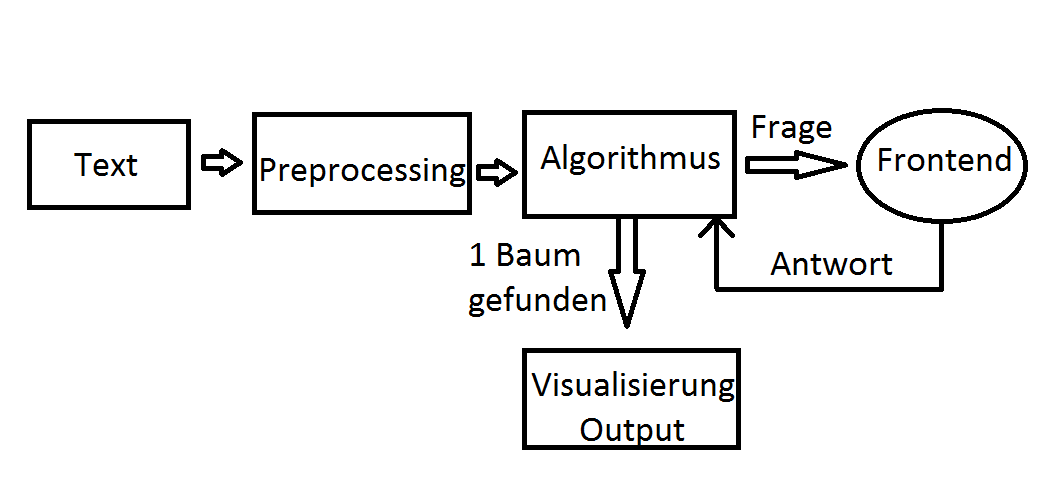
\includegraphics[scale=0.4]{Grafik}
\end{frame}

\begin{frame}
    \frametitle{Algorithmus}
    \begin{itemize}
        \item Generiere aus Parseforest die Frage, welche bei ihrer Beantwortung die meisten Bäume rausfiltert.
            \begin{itemize}
                \item Suche des Tupels, das den Suchraum am ehesten halbiert:
            \end{itemize}
    \end{itemize}
    \begin{algorithmic}
        \State a $\gets$ len(parses) \Comment Anzahl der Parse-Bäume.
        \For{each tuple}
        \State score $\gets$ $\mathrm{abs}(\mathrm{count(tuple)} - \frac{a}{2})$
        \EndFor
    \end{algorithmic}
    \begin{itemize}
        \item Nimm den Tupel als Frage
    \end{itemize}
\end{frame}

\begin{frame}
    \frametitle{Abhängigkeiten}
    \begin{itemize}
        \item Python 3.4 order neuer (aufgrund des Pakets \texttt{asyncio})
        \item Parser, der k-best Parses liefert
        \item TCP- oder UNIX-Sockets
        \item JSON
    \end{itemize}
\end{frame}

\begin{frame}
    \frametitle{Client-Server-Kommunikation I}
    \begin{itemize}
        \item Client und Server kommunizieren streambasiert über eine offen gehaltene Verbindung.
        \item Das geschieht entweder über ein TCP- oder ein UNIX-Socket.
        \item Jede Nachricht besteht aus genau einem JSON-Objekt, das den Schlüssel \texttt{"type"} enthalten muss.
        \item Es gibt die fünf Typen \texttt{request}, \texttt{question}, \texttt{answer}, \texttt{solution} und \texttt{error}.
    \end{itemize}
\end{frame}

\begin{frame}
    \frametitle{Client-Server-Kommunikation II}
    \centering
    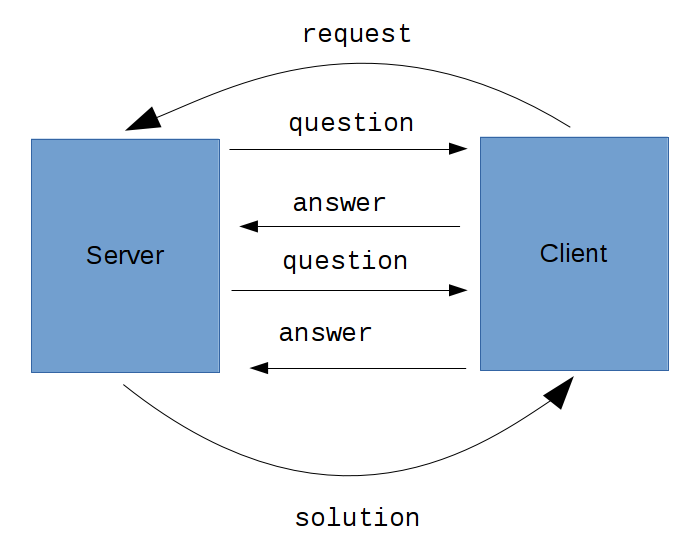
\includegraphics[scale=0.4]{server_client.png}
\end{frame}

\begin{frame}
    \frametitle{Nachricht des Typs \texttt{request}}
    \begin{itemize}
        \item Ein \texttt{request} wird vom \emph{Client} gestellt, um die Annotation eines Satzes einzuleiten.
        \item Der Client spezifiziert ein Feld außer dem \texttt{type}:
            \begin{description}
                \item[\texttt{use\_forest}] wenn der Server einen schon in einen Wald geparsten Satz verwenden soll.
                    Der Wert des Feldes soll dann eine CoNLL-Repräsentation des Waldes sein.
                \item[\texttt{parse\_sentence}] wenn der Server den angegebenen Satz selbst parsen soll.
                    Der Wert des Feldes soll dann ein ganz normaler Satz sein.
            \end{description}
    \end{itemize}
\end{frame}

\begin{frame}
    \frametitle{Beispiel: \texttt{request} mit \texttt{parse\_sentence}}
    \lstinputlisting{request_parse_sentence.json}
\end{frame}

\begin{frame}
    \frametitle{Beispiel: \texttt{request} mit \texttt{use\_forest}}
    \lstinputlisting{request_use_forest.json}
\end{frame}

\begin{frame}
    \frametitle{Nachricht des Typs \texttt{question}}
    \begin{itemize}
        \item Hat der Server eine Frage gefunden, die er dem Client stellen will, sendet er eine Nachricht des Typs \texttt{question}.
        \item Der Server spezifiziert außer dem \texttt{type} die folgenden Felder:
            \begin{description}
                \item[\texttt{question}] Eine Repräsentation der Frage
                    Der Wert des Feldes steht noch nicht völlig fest, ist er wohl ein weiteres JSON-Objekt.
                \item[\texttt{remaining\_trees}] Ein Integer, der angibt, wie viele Bäume noch im Wald enthalten sind.
                \item[\texttt{sentence}] Ein String, der den behandelten Satz enthält.
                \item[\texttt{fixed\_edges}] Ein Array von Edge-Objekten, die die Kanten repräsentieren, die in jedem Baum im Wald vorkommen und daher schon feststehen.
            \end{description}
    \end{itemize}
\end{frame}

\begin{frame}
    \frametitle{Beispiel: \texttt{question}}
    \lstinputlisting{question.json}
\end{frame}

\begin{frame}
    \frametitle{Nachricht des Typs \texttt{answer}}
    \begin{itemize}
        \item Hat der Client auf die Frage des Servers eine Antwort gefunden, sendet er eine Nachricht des Typs \texttt{answer}.
        \item Der Client spezifiziert außer dem \texttt{type} die folgenden Felder:
            \begin{description}
                \item[\texttt{question}] Ein Edge-Objekt, das der Client bestätigen oder zurückweisen soll.
                \item[\texttt{answer}] Ein boolescher Wert, der die Frage beantwortet, d. h. die vom Server genannte Kante bestätigt oder zurückweist.
            \end{description}
    \end{itemize}
\end{frame}

\begin{frame}
    \frametitle{Beispiel: \texttt{answer}}
    \lstinputlisting{answer.json}
\end{frame}

\begin{frame}
    \frametitle{Nachricht des Typs \texttt{solution}}
    \begin{itemize}
        \item Hat sich der Wald so weit gelichtet, dass nur noch ein Baum übrig ist, sendet der Server keine weitere Frage, sondern eine Nachricht des Typs \texttt{solution}.
        \item Der Client spezifiziert außer dem \texttt{type} das folgende Feld:
            \begin{description}
                \item[\texttt{tree}] Eine Repräsentation des übrig gebliebenen Baumes.
                    Der Wert des Feldes steht noch nicht völlig fest, ist er wohl ein weiteres JSON-Objekt.
            \end{description}
    \end{itemize}
\end{frame}

\begin{frame}
    \frametitle{Beispiel: \texttt{solution}}
    \lstinputlisting{solution.json}
\end{frame}

\begin{frame}
    \frametitle{Nachricht des Typs \texttt{error}}
    \begin{itemize}
        \item Empfängt der Server vom Client eine unerwartete Nachricht, so antwortet er mit einer Nachricht vom Typ \texttt{error}.
        \item Der Client spezifiziert außer dem \texttt{type} folgende Felder:
            \begin{description}
                \item[\texttt{error\_message}] Ein String, der den Fehler beschreibt.
                \item[\texttt{recommendation}] Ein String, der eine Empfehlung an den Client ausspricht, wie er den Fehler behandeln soll.
                    Mögliche Werte werden vermutlich \texttt{"retry"} und \texttt{"abort"} sein.
            \end{description}
    \end{itemize}
\end{frame}

\begin{frame}
    \frametitle{Beispiel: \texttt{error}}
    \lstinputlisting{error.json}
\end{frame}

\section{Features}

\begin{frame}
    \frametitle{Features – Pflicht}
    \begin{itemize}
        \item  Stellen von Fragen  der Form: „Ist Token1 Relation von Token2?“ an den Annotator
        \item Antwort reduziert Anzahl der möglichen Parsebäume bis nur noch einer übrig ist
        \item fertiger Parsebaum wird dem Nutzer gezeigt
        \item Nutzer kann Parsebaum abspeichern
    \end{itemize}
\end{frame}

\begin{frame}
    \frametitle{Features – Optional}
    Die Erstellung eines interaktiven GUIs, welches den bisherigen Parsebaum anzeigt und weitere benutzerfreundliche Features anbietet:
    \begin{itemize}
        \item Eine \emph{Undo}-Taste um Fehler zu korrigieren.
        \item Ein visueller Hinweis darauf, welche Felder des Parsebaums bereits feststehen. Der Annotator erkennt somit frühzeitig, falls eine bestimmte Annotation vom System garnicht betrachtet wird.
    \end{itemize}
\end{frame}

\begin{frame}
    \frametitle{Features – Optional}
    \begin{itemize}
        \item Implementierung weiterer Algorithmen zur Fragengenerierung.
        \item Eine breitere Formatsunterstützung bei der Ausgabe der fertigen Parsebäume.
    \end{itemize}
\end{frame}

\section{Evaluation}

\begin{frame}
    \frametitle{Evaluation}
    \begin{itemize}
        \item Automatische Evaluation
            \begin{itemize}
                \item Methode:
                    \begin{itemize}
                        \item der Goldparse wird als Annotator benutzt
                        \item die Fragen werden an den Goldpars gestellt
                        \item überprüfen: Entspricht Ergebnis dem Goldpars?
                    \end{itemize}
                \item Vorteile
                    \begin{itemize}
                        \item Überprüfen mehrerer Ergebnisse in derselben Zeit
                        \item Vermeiden menschlicher Fehler
                    \end{itemize}
            \end{itemize}
    \end{itemize}
\end{frame}

\begin{frame}{Evaluationsmaß}
    \begin{itemize}
        \item mehrere Evaluationsmaße
            \begin{itemize}
                \item Minimum Edit Distance
                    \begin{itemize}
                        \item Anzahl der nicht übereinstimmenden, gelabelten Kanten
                    \end{itemize}
                \item Labeled Attachment Score
                    \begin{itemize}
                        \item Anzahl der gelabeled Kanten, die mit dem Goldstandard übereinstimmen
                    \end{itemize}
                \item Error Counter
                    \begin{itemize}
                        \item Anzahl der nicht gefundenen Bäume
                    \end{itemize}
            \end{itemize}
    \end{itemize}
\end{frame}
\end{document}
